% ============================================================
% Inference-Time Acoustic Style Transfer in F5-TTS
% Signal Processing & Learning Methods for Speech — Final Project
% Tel Aviv University
% ============================================================

\PassOptionsToPackage{unicode}{hyperref}
\PassOptionsToPackage{hyphens}{url}

\documentclass[11pt,a4paper,twocolumn]{article}

% ── Core packages ──────────────────────────────────────────
\usepackage{amsmath,amssymb,amsfonts}
\usepackage{lmodern}
\usepackage[T1]{fontenc}
\usepackage[utf8]{inputenc}
\usepackage{textcomp}
\usepackage{microtype}
\usepackage{graphicx}
\usepackage{xcolor}
\usepackage{booktabs}
\usepackage{array}
\usepackage{caption}
\usepackage{gensymb}
\usepackage{tikz}
\usetikzlibrary{arrows.meta, positioning, fit, backgrounds}

% ── Equation overflow fix ───────────────────────────────────
\relpenalty=9999
\binoppenalty=9999
\usepackage[normalem]{ulem}
\usepackage[margin=2.5cm]{geometry}
\usepackage{setspace}
\usepackage{parskip}
\usepackage{float}
\usepackage{placeins}
\usepackage{subcaption}
\usepackage{enumitem}
\usepackage[hidelinks]{hyperref}
\usepackage{bookmark}

% ── Hyperref metadata ──────────────────────────────────────
\hypersetup{
  pdftitle={Inference-Time Acoustic Style Transfer in F5-TTS via Mel
            Conditioning Interpolation and Flow-Matching Initialisation Biasing},
  pdfkeywords={text-to-speech, style transfer, flow matching, SDEdit, F5-TTS},
  hidelinks
}

% ── Image scaling ──────────────────────────────────────────
\makeatletter
\def\maxwidth{\ifdim\Gin@nat@width>\linewidth\linewidth\else\Gin@nat@width\fi}
\def\maxheight{\ifdim\Gin@nat@height>\textheight\textheight\else\Gin@nat@height\fi}
\makeatother
\setkeys{Gin}{width=\maxwidth,height=\maxheight,keepaspectratio}

% ── Caption style ──────────────────────────────────────────
\captionsetup{font=small, labelfont=bf, justification=justified,
              skip=4pt, width=0.95\linewidth}

% ── Misc ───────────────────────────────────────────────────
\setlength{\emergencystretch}{3em}
\setcounter{secnumdepth}{3}

% ── Title ──────────────────────────────────────────────────
\title{\Large\bfseries
  Inference-Time Acoustic Style Transfer in F5-TTS\\[4pt]
  via Mel Conditioning Interpolation\\
  and Flow-Matching Initialisation Biasing}

\author{
 \textit{N. Dahan, Y. Carmel}\\
  \textit{Signal Processing \& Learning Methods for Speech}\\
  \textit{School of Electrical Engineering,}\\
  \textit{Tel Aviv University}
}

\date{February 2026}

% ============================================================
\begin{document}
\twocolumn[{%
\begin{@twocolumnfalse}
\maketitle

% ── Abstract ───────────────────────────────────────────────
\begin{abstract}
\noindent
F5-TTS~\cite{chen2025f5tts} is a state-of-the-art zero-shot text-to-speech
system based on Conditional Flow Matching (CFM) and Diffusion Transformers.
Despite its impressive voice-cloning capability, the paper explicitly
identifies the absence of fine-grained paralinguistic control—particularly
emotion—as a key limitation.  We reproduce the paper's sway-sampling and
classifier-free guidance ablations, confirming that $s{=}{-}0.8$, NFE$=32$
achieves 0\,\% word error rate.  We then introduce two complementary
inference-time extensions that require no retraining.
\textbf{Extension\,1} injects a linearly interpolated blend of two reference
mel spectrograms directly into the model's conditioning branch, producing a
smooth acoustic gradient between speakers measurable via speaker similarity
and mel-cepstral distortion.
\textbf{Extension\,2} adapts the SDEdit (stochastic differential edit) framework~\cite{song2022sdedit} to
flow-matching TTS by biasing the ODE starting point toward a style reference
while conditioning on an identity reference; four variants are evaluated:
SDEdit initialisation (A), style guidance via a two-pass ODE (B),
scheduled conditioning switching (C), and noise statistics transfer (D).
We discuss why extending F5-TTS to unseen languages such as Hebrew requires
full retraining, and analyse a novel security concern: the noise
initialisation channel, once exposed as a controllable interface, constitutes
a potential adversarial injection surface.

\medskip\noindent
\textbf{Keywords:} text-to-speech; acoustic style transfer; flow matching;
SDEdit; mel spectrogram; paralinguistic control; adversarial examples.
\end{abstract}
\vspace{\baselineskip}
\end{@twocolumnfalse}%
}]
\thispagestyle{empty}

% ============================================================
\section{Introduction}
\label{sec:intro}
% ============================================================

Zero-shot voice cloning—generating speech in an arbitrary speaker's voice
from a short reference clip without speaker-specific training—has advanced
rapidly through the adoption of diffusion and flow-matching
generative models~\cite{lipman2023flow,ho2020ddpm}.
F5-TTS~\cite{chen2025f5tts} pushes this paradigm with a fully
non-autoregressive Diffusion Transformer (DiT) conditioned on reference mel
spectrograms, achieving near-perfect transcription accuracy with 32 neural
function evaluations.

Despite these gains, F5-TTS's own conclusion notes a critical gap:
\emph{``F5-TTS lacks fine-grained control of paralinguistic details,
e.g.\ emotion.''}~\cite{chen2025f5tts}.
The model can replicate \emph{who} is speaking but cannot independently
control \emph{how} they speak—their emotional tone, energy, or prosodic style.
Addressing this gap is the central motivation of this work.
We use ``style transfer'' broadly to encompass any inference-time
manipulation that shifts the acoustic characteristics of generated speech
toward a reference signal---including acoustic morphing where identity and
style are not fully disentangled.

We make the following contributions:
\begin{enumerate}[leftmargin=*,label=(\arabic*)]
  \item \textbf{Baseline reproduction}: we replicate the sway-sampling and
    CFG strength ablations from the original paper, validating our pipeline.
  \item \textbf{Direct mel injection} (Extension 1): we expose a dormant 3D
    conditioning branch in \texttt{cfm.py} that accepts mel spectrograms
    directly, bypassing the vocoder, and use it to blend two reference
    speakers' conditioning mels at inference time.
  \item \textbf{Noise-biased style transfer} (Extension 2): four
    inference-time methods: (A)~biasing the ODE starting noise toward a
    style reference's mel; (B)~steering the vector field via a two-pass
    style guidance term; (C)~switching the conditioning mel from style to
    identity at a scheduled ODE timestep; (D)~transferring the style
    reference's global amplitude statistics onto the initial noise.
  \item A discussion of cross-lingual limitations (Hebrew) and a novel adversarial threat model enabled by the noise initialisation interface.
\end{enumerate}

All experiments use the publicly available pretrained F5-TTS checkpoint.
No fine-tuning or model modification (beyond the \texttt{cfm.py} extension)
is performed.
Due to the exploratory nature of this project, all experiments use a small
evaluation set (three sentences, one speaker pair).

% ============================================================
\section{Background}
\label{sec:background}
% ============================================================

\subsection{Conditional Flow Matching}
\label{sec:cfm}

F5-TTS generates mel spectrograms by solving an ODE:
\begin{align}
  &\frac{d\psi_t(x_0)}{dt} = v_t\!\bigl(\psi_t(x_0),\,c\bigr),\notag\\
  &\psi_0(x_0)=x_0,\quad \psi_1(x_0)=x_1,
  \label{eq:ode}
\end{align}
where $x_0\sim\mathcal{N}(0,I)$ is sampled noise,
$x_1$ is the target mel spectrogram,
$v_t$ is a DiT vector field, and
$c=(x_{\mathrm{ref}},\,z_{\mathrm{ref{\cdot}gen}})$ is the conditioning
(reference mel concatenated with the character sequence along the time axis).
Training uses the Conditional Flow Matching objective~\cite{lipman2023flow},
which directly regresses the ground-truth transport vector field without
requiring a DDPM noise schedule~\cite{ho2020ddpm}.

Classifier-free guidance~\cite{ho2022cfg} is applied during inference:
\begin{align}
  v_{\rm guided} &= v_t(x,\varnothing)\notag\\
    &\quad+ \lambda\bigl[v_t(x,c)-v_t(x,\varnothing)\bigr],
  \label{eq:cfg}
\end{align}
where $\varnothing$ denotes a dropped (null) conditioning and $\lambda$ is
the guidance strength.

\subsection{Sway Sampling}
\label{sec:sway}

F5-TTS replaces the uniform ODE timestep grid with a non-uniform schedule
\begin{equation}
  t' = t + s\!\left(\cos\!\tfrac{\pi}{2}t - 1 + t\right),
  \label{eq:sway}
\end{equation}
which, for $s<0$, concentrates function evaluations near the noisy end
$(t\approx 0)$.  The paper demonstrates that $s=-1$ with NFE$=32$ minimises
WER~\cite{chen2025f5tts}.

\subsection{Evaluation Metrics}
\label{sec:metrics}

Three complementary metrics are used throughout:
\textbf{WER} (word error rate) via Whisper large-v3-turbo~\cite{radford2023whisper}
measures intelligibility.
\textbf{SIM} (speaker similarity), computed as the cosine similarity of
mean-pooled WavLM-Base-Plus~\cite{chen2022wavlm} embeddings, measures
how closely the generated audio matches a reference speaker.
In single-reference experiments we write SIM-o (similarity to the sole
conditioning reference); where two references are active, SIM-A denotes
similarity to the identity reference and SIM-B to the style reference.
\textbf{MCD} (mel-cepstral distortion, 24 MFCCs, DTW-aligned) measures
acoustic distance from a reference in cepstral space.

% ============================================================
\section{Baseline Reproduction}
\label{sec:baseline}
% ============================================================

\subsection{Sway Sampling Ablation}

We reproduced the sway-sampling experiment from Fig.\,3 / Table\,2 of the
base article over $s \in \{+0.4, 0.0, -0.4, -0.8, -1.0\}$ and
NFE $\in \{8, 16, 32\}$, for three test sentences (45 inferences total).
Table~\ref{tab:sway} reports WER averaged across sentences for selected
$s$--NFE combinations.

\begin{center}
\captionof{table}{Sway sampling ablation: mean WER (\%) and SIM-o over
three sentences. Best result per NFE shown in \textbf{bold}.}
\label{tab:sway}
\smallskip
\setlength{\tabcolsep}{4pt}
\begin{tabular}{@{}ccrr@{}}
\toprule
$s$ & NFE & WER\,(\%) & SIM-o  \\
\midrule
$+0.4$ & 8  & 87.9 & 0.694 \\
$+0.4$ & 32 & 51.9 & 0.827  \\
$0.0$  & 32 &  3.7 & 0.836  \\
$-0.4$ & 32 &  7.9 & 0.826  \\
$-0.8$ & 32 & \textbf{0.0} & 0.784  \\
$-1.0$ & 8  & \textbf{20.7} & 0.830  \\
$-1.0$ & 32 &  7.4 & 0.802  \\
\bottomrule
\end{tabular}
\end{center}

Key finding: $s=-0.8$ with NFE$=32$ achieves 0\,\% WER on all three
sentences.  This differs slightly from the original paper's reported
optimum of $s=-1$ (which yields 7.4\,\% WER in our reproduction),
likely due to our smaller test set.  At NFE$=8$, the
bias of $s=-1.0$ provides the largest benefit (+67 pp WER reduction vs.\
$s=+0.4$), confirming that biased sampling is most valuable in the
low-step budget regime.  Figure~\ref{fig:sway_pdf} illustrates the
resulting timestep densities.

\begin{figure}[htbp]
  \centering
  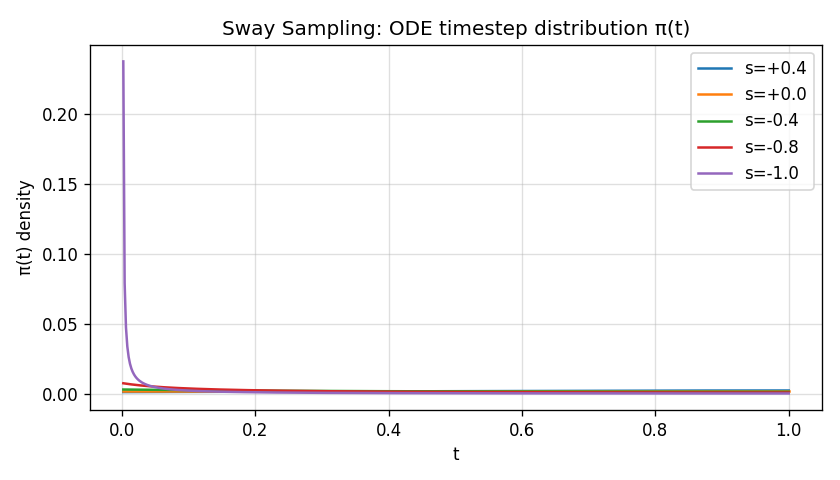
\includegraphics[width=\linewidth]{results/plots/sway_pdf.png}
  \caption{ODE timestep probability densities for each sway coefficient.
  Negative $s$ concentrates evaluations near $t=0$ (the noisy end);
  the shape matches Fig.\,2 of the base article.}
  \label{fig:sway_pdf}
\end{figure}


\begin{figure}[htbp]
  \centering
  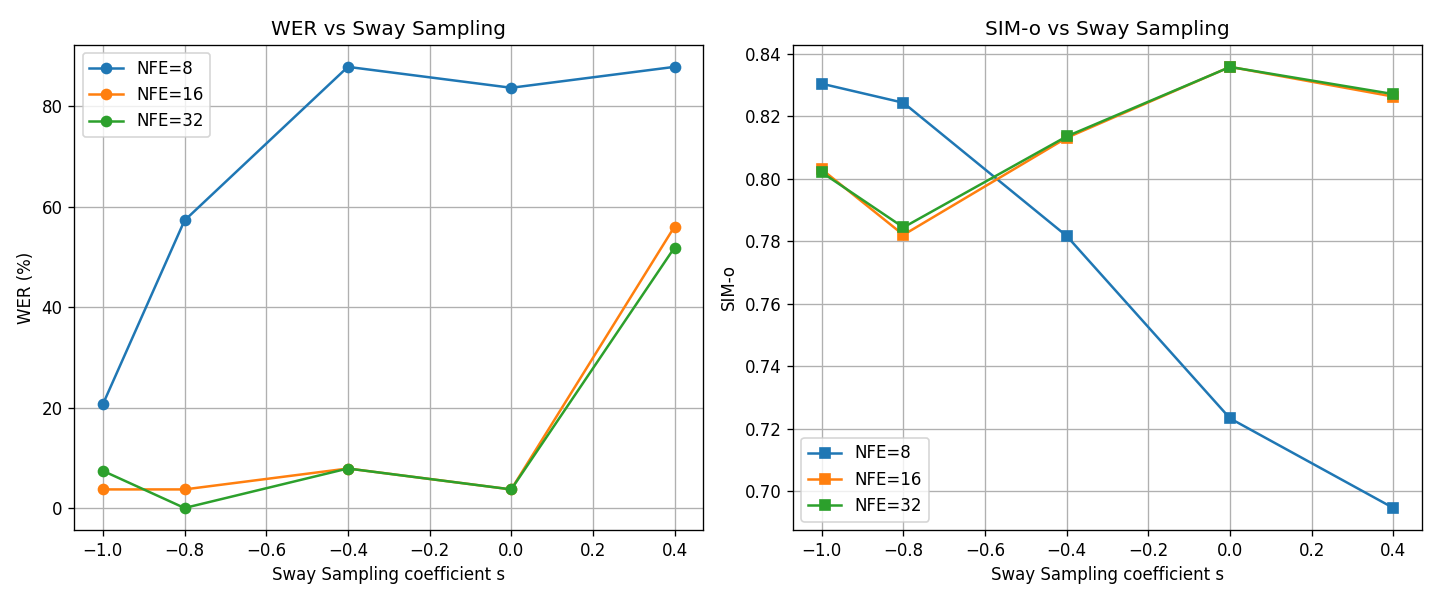
\includegraphics[width=\linewidth]{results/plots/sway_sampling.png}
  \caption{WER and SIM-o vs.\ sway coefficient for NFE$\in\{8,16,32\}$.
  The cross-over between NFE curves demonstrates that negative sway
  matters most when fewer ODE steps are taken.}
  \label{fig:sway}
\end{figure}

\subsection{CFG Strength Ablation}

Table~\ref{tab:cfg} sweeps $\lambda \in \{1.0,1.5,2.0,2.5,3.0\}$ at
fixed $s=-1.0$, NFE$=32$.  WER improves monotonically with stronger
guidance, while SIM-o peaks at $\lambda=1.0$--$1.5$ and then falls.
The paper's default $\lambda=2.0$ (WER\,=\,7.4\,\%, SIM-o\,=\,0.802)
sits at the elbow of this trade-off.

\begin{center}
\captionof{table}{CFG strength ablation: mean WER (\%) and SIM-o.}
\label{tab:cfg}
\smallskip
\setlength{\tabcolsep}{4pt}
\begin{tabular}{@{}crr@{}}
\toprule
$\lambda$ & WER\,(\%) & SIM-o \\
\midrule
1.0 & 17.2 & 0.835 \\
1.5 & 11.1 & 0.821 \\
2.0 &  7.4 & 0.802 \\
2.5 &  3.7 & 0.756 \\
3.0 &  3.7 & 0.774 \\
\bottomrule
\end{tabular}
\end{center}

\begin{figure}[htbp]
  \centering
  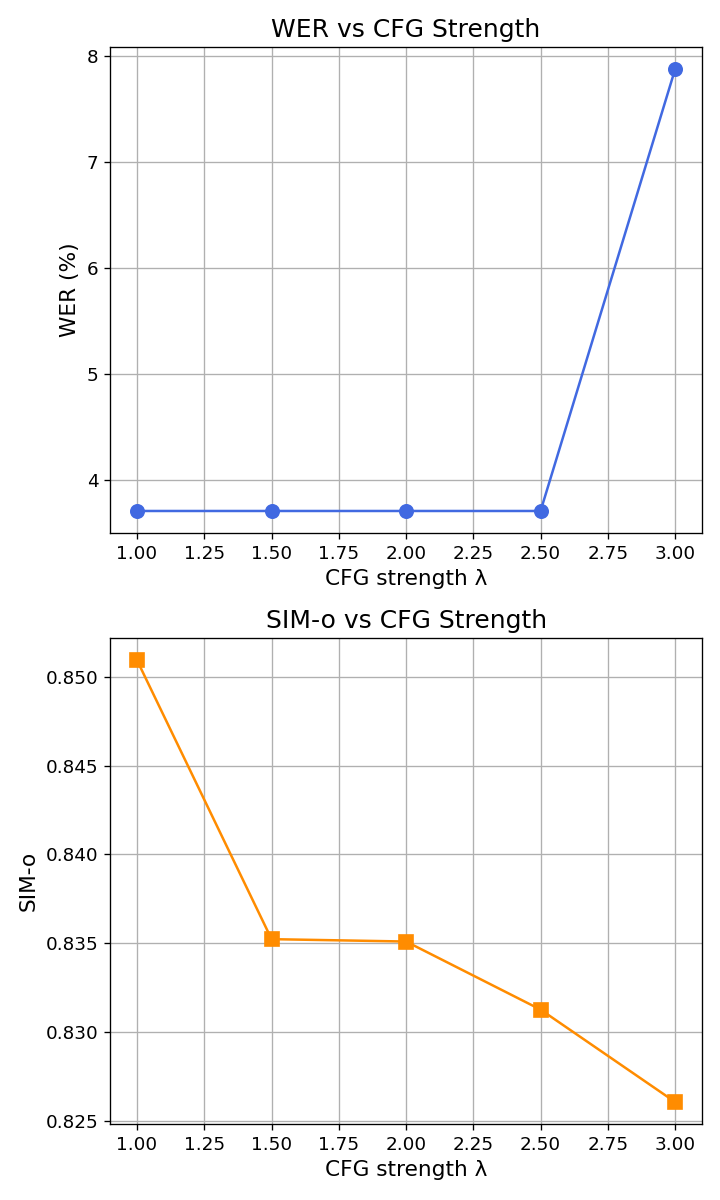
\includegraphics[width=\linewidth]{results/plots/cfg_strength.png}
  \caption{CFG strength ablation: WER decreases and SIM-o peaks at
    $\lambda\approx1.0$--$1.5$ before falling, confirming $\lambda=2.0$
    as a good operating point.}
  \label{fig:cfg}
\end{figure}

% ============================================================
\section{Extension 1: Direct Mel Conditioning Interpolation}
\label{sec:ext1}
% ============================================================

\subsection{Motivation and Architecture Insight}

F5-TTS conditions the DiT on a reference mel by concatenating it (time-axis)
to the noisy input.  Inspection of \texttt{cfm.py} (lines 106--109) reveals
a dormant branch:
\begin{equation*}
\texttt{if cond.ndim == 2:}\;\text{convert waveform}\rightarrow\text{mel}
\end{equation*}
When a 3D tensor \texttt{cond} $\in\mathbb{R}^{B\times T\times 100}$ is
passed, the conversion is skipped entirely—the caller supplies the mel
directly.  This interface, present in the published codebase but unexploited
in the official CLI, enables us to inject \emph{arbitrary} mel tensors as
conditioning with zero architectural change.

\subsection{Mel Blending}

Given identity reference $A$ and style reference $B$ with mels
$\mathbf{m}_A, \mathbf{m}_B \in\mathbb{R}^{T\times 100}$ (computed via
the model's own \texttt{MelSpec} module to remain in-distribution), we form
\begin{equation}
  \mathbf{m}{(\alpha)} = (1-\alpha)\,\mathbf{m}_A + \alpha\,\mathbf{m}_B,
  \quad \alpha\in[0,1].
  \label{eq:blend}
\end{equation}
Because both mels are computed by the identical mel filterbank the model was
trained with (24\,kHz, 100 channels, hop\,=\,256, Slaney norm), the blended
tensor is in-distribution for the transformer even if novel as a conditioning
signal.

\textbf{Why not blend waveforms or invert first?}
Waveform mixing causes phase interference that destroys spectral structure.
Blending in mel space then inverting via Vocos fails at intermediate weights:
a linearly blended mel is out-of-distribution for the vocoder, producing
clipped, ~1\,s garbled outputs (100\,\% WER at $\alpha\in(0.1,0.9)$ in our v1
experiments).  Direct 3D injection bypasses Vocos inversion entirely.

\textbf{Important limitation.}
A mel spectrogram encodes identity (vocal tract shape, voice quality),
prosody (pitch, rate, energy), and emotional style \emph{jointly}.
Linear blending therefore produces an acoustic morph between the two
speakers—not ``A's voice with B's emotion.''  True identity-preserving
emotion transfer would require a disentangled representation (separate
speaker and emotion encoders) that F5-TTS does not possess.

\subsection{Results}

Identity reference\,A: canonical English male demo (\texttt{basic\_ref\_en.wav}).
Style reference\,B: Mandarin animated character (\texttt{basic\_ref\_zh.wav}).
Target text (same for all runs):
\emph{``I don't really care what you call me. I've been a silent spectator,
watching species evolve, empires rise and fall.''}

\begin{center}
\captionof{table}{Direct mel injection results.  SIM-o is cosine similarity
vs.\ reference~A; MCD is mel-cepstral distortion vs.\ A.}
\label{tab:ext1}
\smallskip
\setlength{\tabcolsep}{3pt}
\begin{tabular}{@{}crrrr@{}}
\toprule
$\alpha$ & Dur (s) & WER\,(\%) & SIM-o & MCD \\
\midrule
0.00 & 12.3 &  0.0 & 0.893 & 726 \\
0.25 & 12.3 &  0.0 & 0.896 & 707 \\
0.50 & 12.3 & 15.0 & 0.833 & 870 \\
0.75 & 13.3 &  0.0 & 0.812 & 832 \\
1.00 & 13.3 &  0.0 & 0.811 & 919 \\
\midrule
zero-shot B & 16.9 & 0.0 & 0.840 & 846 \\
\bottomrule
\end{tabular}
\end{center}

\begin{figure}[htbp]
  \centering
  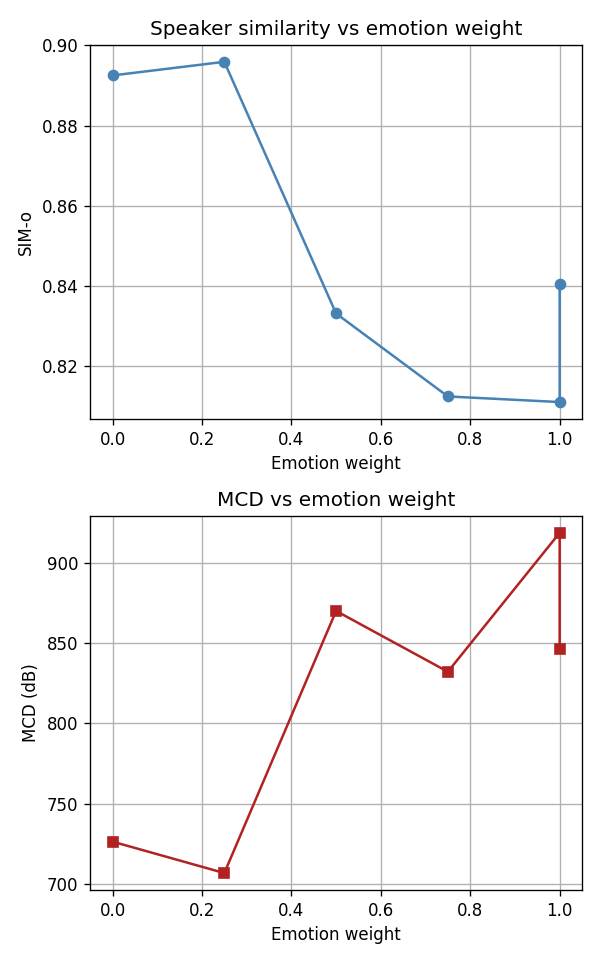
\includegraphics[width=\linewidth]{results/plots/emotion_weight.png}
  \caption{SIM-o and MCD as a function of blend weight $\alpha$.
  Both metrics shift monotonically, confirming a smooth acoustic gradient
  between the two reference speakers.}
  \label{fig:ext1}
\end{figure}

The metric trajectories in Fig.~\ref{fig:ext1} confirm a smooth acoustic
gradient: SIM-o decreases ($A$'s identity is diluted) and MCD increases
(output moves away from $A$) as $\alpha$ grows.  Duration also shifts from
$A$'s pace (12.3\,s) toward $B$'s (13.3\,s) at $\alpha\geq0.75$, reflecting
B's conditioning mel's influence on prosodic rhythm.

The $\alpha=0.5$ artefact (WER\,=\,15\,\%) is noteworthy: reference A's
transcript contains ``Some call me nature...''; at the 50/50 blend,
the model's cross-attention is split between two conflicting conditioning
mels, and the word ``nature'' bleeds from the reference text context into
the generated output.  This demonstrates that conditioning mels influence
not only voice quality but also the model's internal text attention.

% ============================================================
\section{Extension 2: Noise-Biased Style Transfer}
\label{sec:ext2}
% ============================================================

\subsection{Overview}

Extension\,1 manipulates \emph{what the model listens to} (the conditioning).
Extension\,2 takes a fundamentally different approach: leave the conditioning
signal pure (always speaker~$A$) and instead bias the ODE \emph{starting
point} $x_0$ toward speaker~$B$'s acoustic structure.

This mirrors SDEdit~\cite{song2022sdedit}: in image editing, SDEdit corrupts
a target image to a chosen noise level then denoises it under a new prompt.
Here, we corrupt/blend speaker~$B$'s mel with Gaussian noise:
\begin{equation}
  x_0 = (1-\alpha)\,\varepsilon + \alpha\,\mathbf{m}_B,
  \quad \varepsilon\sim\mathcal{N}(0,I),
  \label{eq:sdedit}
\end{equation}
and integrate the ODE from $t_{\rm start}=\alpha$ conditioned throughout
on $\mathbf{m}_A$.  Four methodological variants are studied.

\subsection{Method A — SDEdit Initialisation}

\textbf{Formulation.} Eq.~\eqref{eq:sdedit} with identity conditioning
throughout.

\textbf{Geometric interpretation.}  Biasing $x_0$ toward $\mathbf{m}_B$
places the trajectory's starting point in a neighbourhood of $B$'s mel in
noise space; the identity conditioning then acts as a gravitational pull
reorienting the trajectory toward $A$'s data manifold.  The trade-off is
controlled by $\alpha$: at small $\alpha$ the effect is subtle; at large
$\alpha$ the model must ``undo'' $B$'s structure with only $1-\alpha$
integration time, degrading intelligibility.

\textbf{Results.}  We performed a fine-grained grid search over
$\alpha\in\{0.00, 0.05, \ldots, 0.70\}$ (step\,0.05) and
$s\in\{-1.0, -0.9, \ldots, +1.0\}$ (step\,0.1), yielding 315 inferences.
The WER–SIM-B trade-off is illustrated in Fig.~\ref{fig:tradeoff}.
The optimal operating point (WER\,=\,0\,\%, maximum SIM-B) is at
$\alpha=0.05$, $s=-0.9$: WER\,=\,0\,\%, SIM-A\,=\,0.874, SIM-B\,=\,0.783,
MCD\,=\,721.9 (vs.\ baseline SIM-B\,=\,0.771 at $\alpha=0$).
Style leakage from $B$ is modest but measurable; beyond $\alpha>0.2$,
WER degrades rapidly (40--100\,\%) as $B$'s temporal structure dominates
the initialisation.

Critically, positive sway ($s>0$) degrades intelligibility even at
$\alpha=0$ (WER exceeds 30\,\% at $s\geq+0.1$, reaching 100\,\% at
$s\geq+0.6$), confirming that concentrating ODE evaluations near $t=1$
(the clean end) is harmful regardless of initialisation.

\begin{figure}[htbp]
  \centering
  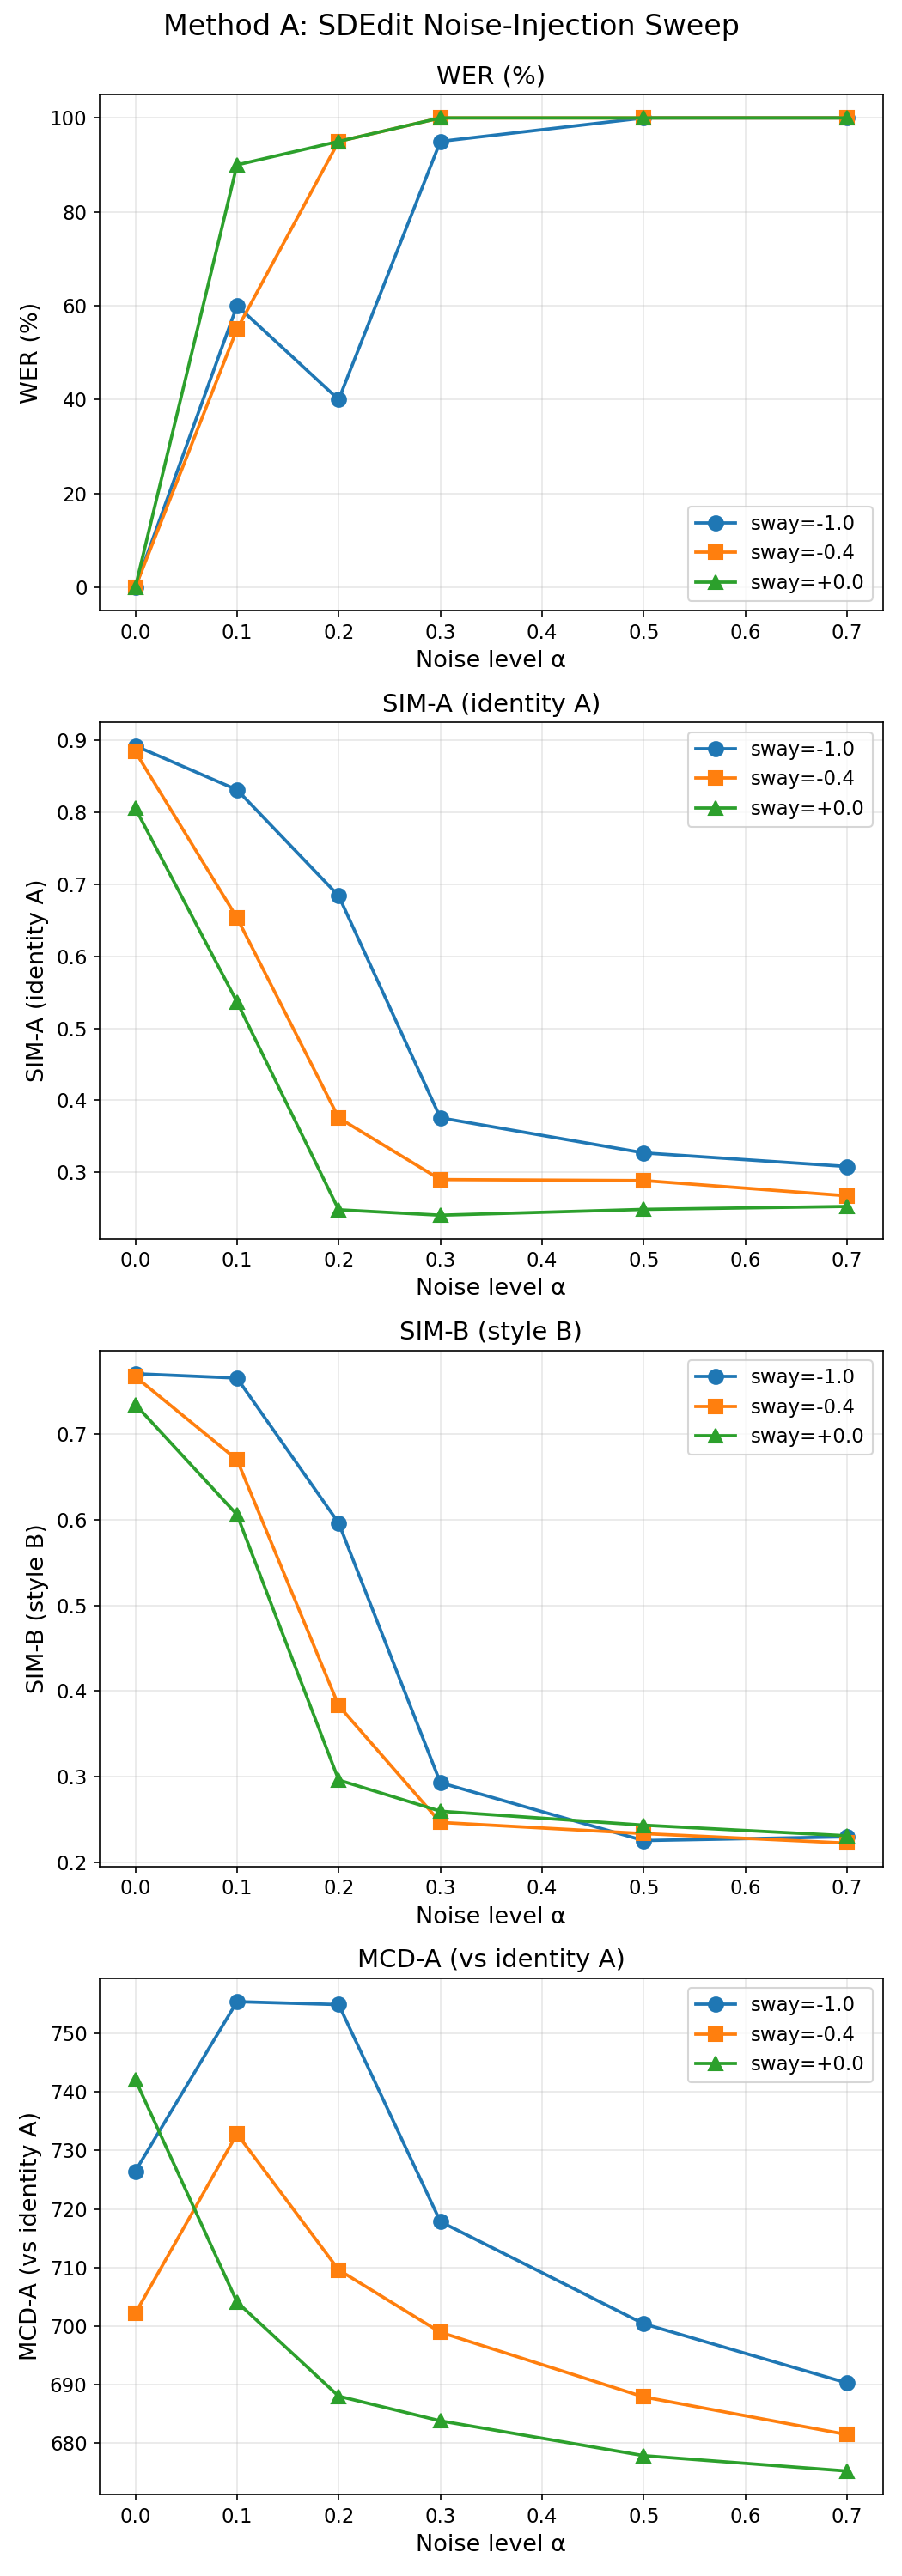
\includegraphics[width=\linewidth]{results/noise_inject/noise_inject_sweep.png}
  \caption{Method~A four-metric sweep: WER, SIM-A, SIM-B, and MCD-A
    as functions of $\alpha$ for $s\in\{-1.0,-0.4,0.0\}$.
    WER begins rising sharply at $\alpha>0.1$ for all sway values.}
  \label{fig:sweep}
\end{figure}

\begin{figure}[htbp]
  \centering
  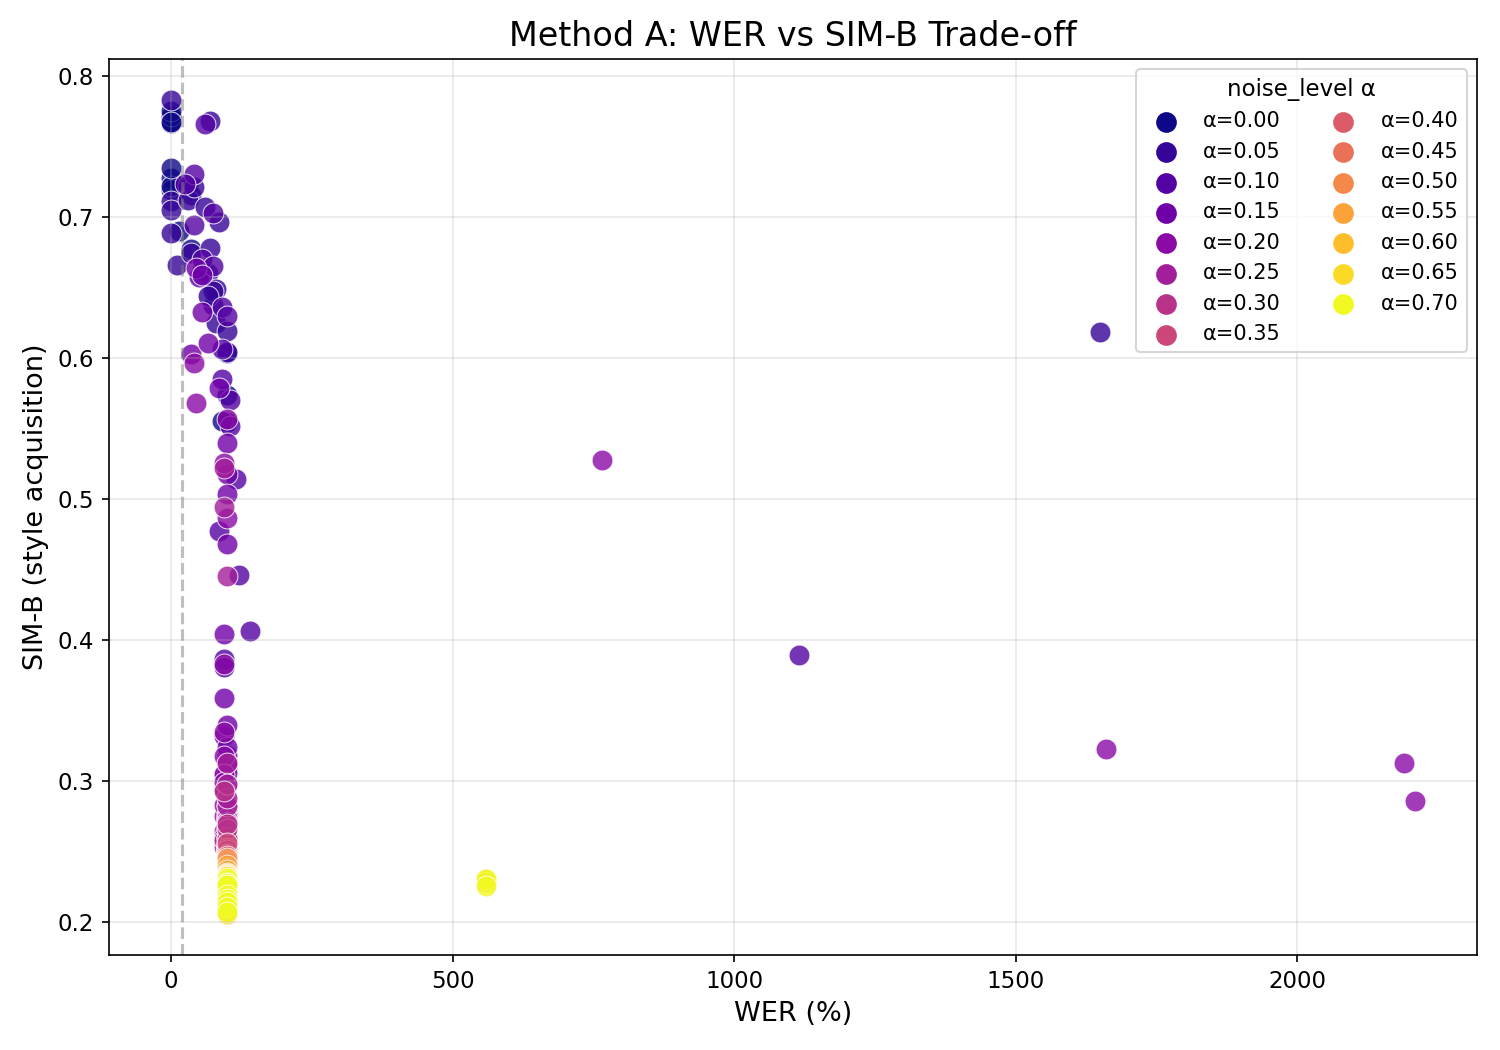
\includegraphics[width=\linewidth]{results/noise_inject/method_A/tradeoff_wer_simb.png}
  \caption{Method~A: WER vs.\ SIM-B scatter for all $(\alpha, s)$ pairs in the
  fine-grained sweep.  Each point is one inference; colour encodes $\alpha$.
  The Pareto-optimal region (low WER, high SIM-B) is at small positive
  $\alpha$ with negative sway.}
  \label{fig:tradeoff}
\end{figure}


\subsection{Method B — Style Guidance (2-Pass ODE)}

\textbf{Formulation.}
At each ODE step the transformer is evaluated twice:
\begin{equation}
  v_{\rm style} = v_A + g\,(v_B - v_A),
  \label{eq:methb}
\end{equation}
where $v_A = v_{\rm guided}(x,\mathbf{m}_A,t)$ and
$v_B = v_{\rm guided}(x,\mathbf{m}_B,t)$, and $g$ is the guidance scale.
This is structurally identical to classifier-free guidance
(Eq.~\ref{eq:cfg}), with $\mathbf{m}_A$ playing the role of the
unconditional baseline.  The computational cost doubles (2$\times$
transformer evaluations per step).

\textbf{Results.} We swept $g\in\{0.25,0.5,0.75,1.0,1.5\}$.
At $g=0.5$, $s=-1.0$: WER\,=\,0\,\%, SIM-A\,=\,0.843,
SIM-B\,=\,\textbf{0.858}, MCD\,=\,809. SIM-B rises by $+0.087$ above
baseline with zero intelligibility loss—the best style transfer of all four
methods.  At $g\geq1.0$ intelligibility collapses (WER\,$\geq$\,70\,\%) as
the vector field is extrapolated beyond the style manifold.

\subsection{Methods C \& D — Negative Results}

Two additional variants were tested but failed to produce intelligible style
transfer at any non-trivial parameter setting.

\textbf{Method C (Scheduled Conditioning)} switches the conditioning mel from
$\mathbf{m}_B$ to $\mathbf{m}_A$ at a threshold timestep $t^*$:
\begin{equation}
  c(t) = \begin{cases} \mathbf{m}_B & t < t^* \\ \mathbf{m}_A & t \geq t^* \end{cases}
  \label{eq:methc}
\end{equation}
All $t^*>0$ cause severe WER degradation
(20--70\,\%), and informal listening confirms the model adopts $B$'s voice
wholesale rather than borrowing stylistic attributes—identity
\emph{replacement}, not style transfer.  The sharp conditioning discontinuity
overwhelms the Euler integrator; a smooth cosine schedule may mitigate this
and is left as future work.

\textbf{Method D (Noise Statistics Transfer)} rescales $x_0$ to match
$\mathbf{m}_B$'s global mean and variance:
\begin{equation}
  x_0 = \frac{\varepsilon}{\|\varepsilon\|_\sigma}\cdot\sigma_{\rm target}
        + \alpha\,\mu_B,
  \label{eq:methd}
\end{equation}
where $\sigma_{\rm target} = \alpha\,\text{std}(\mathbf{m}_B)
+ (1-\alpha)\,\text{std}(\varepsilon)$ and $\mu_B = \text{mean}(\mathbf{m}_B)$.
At all non-zero $\alpha$, WER\,=\,100\,\%.  This strong negative result
reveals that the model is sensitive to the \emph{variance} of $x_0$, not
only its spatial structure: rescaling destroys the implicit amplitude
calibration the ODE integration relies on.

\subsection{Cross-Method Comparison}
\label{sec:comparison}

Table~\ref{tab:comparison} summarises the best intelligibility-preserving
(WER\,=\,0\,\%) result from each method at $s=-1.0$.  Figure~\ref{fig:scatter}
compares the WER–SIM-B scatter across all methods.  Note that Methods~C
and~D achieve WER\,=\,0\,\% only at their trivial settings ($t^*{=}0$ and
$\alpha{=}0$), which reduce to the baseline.

\begin{center}
\captionof{table}{Best WER\,=\,0\,\% result per method at $s=-1$.
Baseline: $\alpha=0$, $g=0$, $t^*=0$.}
\label{tab:comparison}
\smallskip
\setlength{\tabcolsep}{3pt}
\begin{tabular}{@{}lrrrr@{}}
\toprule
Method & WER & SIM-A & SIM-B & MCD \\
\midrule
Baseline          & 0\,\% & 0.893 & 0.771 & 726 \\
A ($\alpha=0.05$) & 0\,\% & 0.874 & 0.783 & 722 \\
B ($g=0.5$)       & 0\,\% & 0.843 & \textbf{0.858} & 809 \\
C ($t^*=0$)       & 0\,\% & 0.893 & 0.771 & 726 \\
D ($\alpha=0$)    & 0\,\% & 0.893 & 0.771 & 726 \\
\midrule
Ext.\,1 ($\alpha=0.25$) & 0\,\% & \multicolumn{2}{c}{SIM-o\,=\,0.896} & 707 \\
\bottomrule
\end{tabular}
\end{center}

\begin{figure}[htbp]
  \centering
  
\includegraphics[width=\linewidth]{results/noise_inject/comparison/comparison_scatter.png}
  \caption{WER vs.\ SIM-B for all inferences across Methods A--D.
  Method~B achieves the highest SIM-B at WER\,=\,0\,\%; Methods~C and~D
  achieve high SIM-B only at the cost of unintelligible output.}
  \label{fig:scatter}
\end{figure}

The comparison reveals a clear hierarchy.  Method~B is the most expressive
($\Delta$SIM-B\,=\,$+0.087$) but requires 2$\times$ compute.  Method~A
provides modest but clean style transfer ($\Delta$SIM-B\,=\,$+0.012$) at
no additional cost.  Methods~C and~D yield high SIM-B figures only in
configurations where speech is unintelligible—hollow wins that do not
represent functional style transfer.  Extension\,1's mel blending is
complementary: it achieves the lowest MCD (707 at $\alpha=0.25$) and the
highest SIM-o, but at the cost of joint identity–style blending rather
than clean style separation.

\subsection{Informal Listening Impressions}
\label{sec:listening}

Two of the authors independently listened to selected samples from each
experiment.  Key observations:
\begin{itemize}[leftmargin=*]
  \item \textbf{Baseline} (Section~\ref{sec:baseline}): intelligible but
    with a slightly robotic, ``phone-call'' quality (naturalness~3/5).
    A noticeable accent shift toward British English was observed relative
    to the American-accented reference.
  \item \textbf{Ext.\,1, $\alpha{=}0$}: near-perfect identity fidelity and
    naturalness (both~5/5); indistinguishable from a standard F5-TTS
    zero-shot output.
  \item \textbf{Ext.\,1, $\alpha{=}0.5$}: a moderate acoustic morph is
    perceptible (3/5), and speech remains fully intelligible (5/5).
    Brief gibberish is audible at the utterance onset, consistent with
    the 15\,\% WER; a faint buzzing artefact persists in the background.
  \item \textbf{Ext.\,1, $\alpha{=}1.0$}: the voice shifts almost entirely
    to reference~B, confirming that identity is not preserved at full
    blend weight (style shift~3/5, naturalness~4/5).
  \item \textbf{Method~A} ($\alpha{=}0.05$, $s{=}{-}0.9$): only a subtle
    difference from the pure baseline is audible (2/5); the output retains
    strong American phonetic features (e.g.\ rhotic /r/) with only a hint
    of reference~B's characteristics.  Fully intelligible (5/5).
  \item \textbf{Method~B} ($g{=}0.5$, $s{=}{-}1$): the most perceptible
    style transfer—the voice retains speaker~A's identity but carries
    reference~B's energy contour and prosodic accent (style acquisition
    3--3.5/5).  Fully intelligible (5/5); minor electronic noise at the
    utterance onset.
  \item \textbf{Method~C} ($t^*{=}0.25$): at sway$=0$ the output is
    partially intelligible (3/5) with noticeable electronic noise
    (naturalness~2/5); at sway$=-1$ intelligibility degrades further.
    In both cases the voice sounds like speaker~B rather than~A
    (style acquisition~4/5), confirming that scheduled conditioning
    produces identity {\em replacement} rather than style transfer—the
    model adopts~B's voice wholesale instead of borrowing only stylistic
    attributes.
  \item \textbf{Method~D}: even at $\alpha{=}0$ (no style injection),
    the output degrades into robotic, distorted speech with heavy
    electrical background noise partway through the utterance.
    At any $\alpha>0$ the output is pure noise.  This confirms the
    quantitative finding: rescaling noise variance disrupts the ODE
    integration so severely that no usable speech is produced.
\end{itemize}
These informal impressions are consistent with the quantitative metrics:
Method~B produces the largest perceptual style shift, matching its
highest $\Delta$SIM-B, while Method~A's modest SIM-B gain corresponds to
a barely perceptible auditory difference.

% ============================================================
\section{Discussion}
\label{sec:discussion}
% ============================================================

\subsection{Cross-Lingual Limitation: Hebrew}%
\label{sec:hebrew}

F5-TTS cannot be applied to Hebrew without substantial retraining.
Its character-level tokeniser (2546 tokens) covers only English and Chinese;
Hebrew characters produce out-of-vocabulary tokens, rendering text
conditioning meaningless.  Even with vocabulary extension, Hebrew phonology
includes sounds absent from both training languages (pharyngeal fricatives,
the approximant \textit{ayin}, the affricate \textit{tsadi}), so the
learned phoneme--acoustic mapping would not generalise.  Our Extensions~1
and~2 operate at the acoustic level and presuppose functional text
conditioning---they cannot compensate for a missing tokeniser.  Meaningful
Hebrew TTS would require tokeniser extension, a large Hebrew speech corpus,
and compute-intensive retraining of the 335\,M-parameter model.

\subsection{A Theoretical Security Concern}%
\label{sec:security}

Extension~2 demonstrates that $x_0$ is a controllable interface.  This
opens a dual-use concern: by analogy with adversarial examples in
discriminative models~\cite{szegedy2014intriguing,goodfellow2015fgsm},
a crafted $x_0$ could steer the generated speech away from what the text
and conditioning specify---e.g.\ injecting unintended content or embedding
covert acoustic commands for downstream voice-activated
systems~\cite{carlini2018audio}.  Method~A already shows that structured
$x_0$ systematically shifts the output; a gradient-optimised variant could
target a specific adversary-chosen mel while appearing statistically
Gaussian.  Mitigations include server-side sampling of $x_0$ from a
cryptographically secure RNG, statistical monitoring of submitted noise
vectors, and output-side safety filters.  We emphasise that this is a
theoretical observation; no attack is attempted.

% ============================================================
\section{Conclusion and Future Work}
\label{sec:conclusion}
% ============================================================

We have demonstrated two families of inference-time acoustic style transfer
for F5-TTS, without modifying model weights.
Extension\,1 (direct mel injection) provides a smooth acoustic gradient
between reference speakers via a dormant but architecturally principled 3D
conditioning branch; it is the simplest intervention and yields the lowest
MCD, though it blends identity and style jointly.
Extension\,2 (noise-biased ODE initialisation) cleanly separates identity
conditioning from style injection; Method~B (2-pass style guidance) achieves
the largest measurable style transfer ($\Delta$SIM-B\,=\,+0.087) at the cost
of doubled inference time, while Method~A provides a cheaper alternative with
modest but zero-WER style leakage.

The comparison of Methods~A--D illuminates the geometry of the flow-matching
ODE: the model is highly sensitive to the \emph{variance} of $x_0$ (Method~D
fails immediately), tolerates frame-level biasing at small $\alpha$ (Method~A),
and can follow a smoothly changing conditioning field provided it is not
switched abruptly (Methods~B vs.\ C).

Several directions remain for future work.
\textbf{Disentangled style transfer:} true emotion-only control requires a
model with separate speaker and emotion encoders; fine-tuning F5-TTS with an
auxiliary emotion classifier loss is one route.
\textbf{Hebrew adaptation:} as argued in Section~\ref{sec:hebrew},
meaningful Hebrew TTS requires tokeniser extension and retraining on a
multilingual corpus—a worthwhile long-term goal as Hebrew speech datasets
grow.
\textbf{Smooth scheduled conditioning:} replacing the step function of
Method~C with a cosine interpolation schedule may recover intelligibility
while retaining the computational efficiency advantage.
\textbf{Adversarial robustness:} the security threat described in
Section~\ref{sec:security} warrants empirical study; gradient-based
optimisation of $x_0$ against a target mel would quantify the practical risk.

% ============================================================
% ============================================================



\begin{thebibliography}{99}

\bibitem{chen2025f5tts}
S.-g.\ Chen, Y.\ Wu, L.\ Wang, Y.\ Liu, and S.\ Watanabe,
``F5-TTS: A Fairytaler that Fakes Fluent and Faithful Speech
with Flow Matching,''
in \textit{Proc.\ ACL 2025}, 2025.
arXiv:2410.06885.

\bibitem{lipman2023flow}
Y.\ Lipman, R.\ T.\ Q.\ Chen, H.\ Ben-Hamu, M.\ Nickel,
and M.\ Le,
``Flow Matching for Generative Modeling,''
in \textit{Proc.\ ICLR 2023}, 2023.
arXiv:2210.02747.

\bibitem{ho2020ddpm}
J.\ Ho, A.\ Jain, and P.\ Abbeel,
``Denoising Diffusion Probabilistic Models,''
in \textit{Proc.\ NeurIPS 2020}, 2020.
arXiv:2006.11239.

\bibitem{song2022sdedit}
C.\ Meng, Y.\ He, Y.\ Song, J.\ Song, J.\ Wu,
J.-Y.\ Zhu, and S.\ Ermon,
``SDEdit: Guided Image Synthesis and Editing with
Stochastic Differential Equations,''
in \textit{Proc.\ ICLR 2022}, 2022.
arXiv:2108.01073.

\bibitem{ho2022cfg}
J.\ Ho and T.\ Salimans,
``Classifier-Free Diffusion Guidance,''
in \textit{NeurIPS 2022 Workshop on DGMs}, 2022.
arXiv:2207.12598.

\bibitem{radford2023whisper}
A.\ Radford, J.\ W.\ Kim, T.\ Xu, G.\ Brockman, C.\ McLeavey,
and I.\ Sutskever,
``Robust Speech Recognition via Large-Scale Weak Supervision,''
in \textit{Proc.\ ICML 2023}, 2023.

\bibitem{chen2022wavlm}
S.\ Chen, C.\ Wang, Z.\ Chen, Y.\ Wu, S.\ Liu, Z.\ Chen,
J.\ Li, N.\ Kanda, T.\ Yoshioka, X.\ Xiao, et al.,
``WavLM: Large-Scale Self-Supervised Pre-Training for Full
Stack Speech Processing,''
\textit{IEEE J.\ Sel.\ Topics Signal Process.},
vol.\ 16, no.\ 6, pp.\ 1505--1518, 2022.
arXiv:2110.13900.

\bibitem{szegedy2014intriguing}
C.\ Szegedy, W.\ Zaremba, I.\ Sutskever, J.\ Bruna,
D.\ Erhan, I.\ Goodfellow, and R.\ Fergus,
``Intriguing Properties of Neural Networks,''
in \textit{Proc.\ ICLR 2014}, 2014.
arXiv:1312.6199.

\bibitem{goodfellow2015fgsm}
I.\ J.\ Goodfellow, J.\ Shlens, and C.\ Szegedy,
``Explaining and Harnessing Adversarial Examples,''
in \textit{Proc.\ ICLR 2015}, 2015.
arXiv:1412.6572.

\bibitem{carlini2018audio}
N.\ Carlini and D.\ Wagner,
``Audio Adversarial Examples: Targeted Attacks on Speech-to-Text,''
in \textit{Proc.\ IEEE Security \& Privacy Workshops (DLS)}, 2018.
arXiv:1801.01944.

\end{thebibliography}

\medskip\noindent
\textbf{Code availability.}\quad
\url{https://github.com/yardencarmel/SigProcForSpeech}

\end{document}
